\documentclass[12pt]{article}

% =========================
% Packages
% =========================
\usepackage[a4paper, margin=1in]{geometry}
\usepackage{amsmath, amssymb, amsfonts}
\DeclareMathOperator{\sech}{sech}
\usepackage{graphicx}
\usepackage{float}
\usepackage{caption}
\usepackage{subcaption}
\usepackage{setspace}
\usepackage{hyperref}
\usepackage{listings}
\usepackage{xcolor}
\lstset{
    language=Matlab,
    basicstyle=\ttfamily\small,
    keywordstyle=\color{blue},
    commentstyle=\color{green!60!black},
    stringstyle=\color{orange},
    numbers=left,
    numberstyle=\tiny,
    stepnumber=1,
    numbersep=5pt,
    frame=single,
    breaklines=true,
    showstringspaces=false,
    tabsize=4
}

\setstretch{1.2}

\begin{document}

\begin{titlepage}
\centering

\vspace*{1.5cm}

% =========================
% Title
% =========================
{\LARGE \textbf{Analysis and Numerical Implementation of a Pseudospectral Method}}\\[0.3cm]

{\large for Head-On Breather Collisions in the Nonlinear Klein-Gordon Equation}

\vspace{1.2cm}

% =========================
% Author + Details
% =========================
{\large Henry Rochester}\\[0.5cm]

{\large
MAM3042F - Advanced Numerical Methods \\[0.3cm]
Department of Mathematics and Applied Mathematics \\ 
University of Cape Town
}

\vspace{1cm}

{\large \today}

\begin{abstract}
In this project, we implement a pseudospectral method to simulate breather solutions of the nonlinear Klein-Gordon equation. We first verify the method on a single breather, which remains localised in space while oscillating in time. We then study head-on collisions between two breathers for different half-separation distances \(d\). The simulations show that the strongest interaction occurs when the breathers are initially superimposed, while for larger values of \(d\), the collision amplitude decreases and then stabilises. Overall, the results show that the initial separation distance affects the strength of the collision most significantly when the breathers begin close together.
\end{abstract}

\end{titlepage}

\section*{Introduction}

We consider the following nonlinear Klein-Gordon equation:
\[
u_{tt} - u_{xx} + 4u - 2u^3 = 0,
\]
subject to periodic boundary conditions:
\[
u(0,t) = u(L,t), 
\qquad 
u_x(0,t) = u_x(L,t).
\]

We note that the spatial profile at the very first moment of time is given by:
\[
u(x,0) = A \cos(kx)\sech\left(\frac{x}{b}\right),
\]
where the parameters \(A\), \(b\), and \(k\) depend on the frequency \(\omega\) and the speed \(v\) of the breather. These are given by: 
\[
A = \frac{2}{\sqrt{3}}
\sqrt{4 - \frac{\omega^2}{1-v^2}},
\]
\[
b = \frac{2}{\sqrt{3}}\frac{\sqrt{1-v^2}}{A},
\]
and
\[
k = \frac{v\omega}{1-v^2}.
\]

Throughout the numerical implementation, we note that we use the parameter values:
\[
\omega = 1.98,
\qquad
v = 0.1.
\]

We are also given that the initial velocity is: 
\[
u_t(x,0)
=
A(\omega + kv)\sin(kx)\sech\left(\frac{x}{b}\right)
+
\frac{Av}{b}
\cos(kx)\sech\left(\frac{x}{b}\right)
\tanh\left(\frac{x}{b}\right).
\]

\section*{Implementation of the Pseudospectral Method}

We first implement the pseudospectral method in code and simulate the solution using the initial condition: 
\[
u(x,0) = A \cos(kx)\sech\left(\frac{x}{b}\right).
\]

We begin by choosing a large value of \(L\). In this implementation, we take
\[
L = 100.
\]
We then choose the number of spatial grid points \(N\) to be a power of \(2\), since the Fast Fourier Transform is most efficient when \(N\) is chosen in this way. We choose $N=512$ here. We then discretise the spatial component of the nonlinear Klein-Gordon equation on the interval:
\[
[-L,L].
\]

The spatial grid is given by:
\[
x_j = -L + jh,
\qquad j = 0,1,\ldots,N-1,
\]
where
\[
h = \frac{2L}{N}.
\]
The corresponding Fourier wavenumbers are thus given by: 
\[
q_n = \frac{\pi n}{L},
\]
where
\[
n = -\frac{N}{2}, \ldots, \frac{N}{2}-1.
\]
We note that since we are working on the interval \([-L,L]\), the spatial period is \(2L\). Hence the Fourier wavenumber is given by: 
\[
\frac{2\pi n}{2L} = \frac{\pi n}{L}.
\]

After discretising in space, the infinite Fourier series representation is truncated. Thus, the numerical scheme that we implement consists of a centered finite difference approximation in time and a truncated Fourier expansion in space. The centered difference approximation for the second time derivative is given by:
\[
u_{tt}(x_j,t_k)
\approx
\frac{u_j^{k+1} - 2u_j^k + u_j^{k-1}}{\tau^2}.
\]

For the spatial derivative, we use the pseudospectral approximation. We note that since we have: 
\[
u(x,t_k)
\approx
\sum_{n=-N/2}^{N/2-1}
\widehat{u}_n(t_k)e^{iq_n x},
\]
then
\[
u_{xx}(x,t_k)
\approx
\sum_{n=-N/2}^{N/2-1}
-q_n^2 \widehat{u}_n(t_k)e^{iq_n x}.
\]
Therefore, at each time step, we compute the Fourier coefficients \(\widehat{u}_n(t_k)\) using the Fast Fourier Transform, multiply each mode by \(-q_n^2\), and then apply the inverse Fast Fourier Transform in order to obtain the values of \(u_{xx}\) at the spatial grid points.

Now recall that the nonlinear Klein-Gordon equation that we are working with is given by: 
\[
u_{tt} - u_{xx} + 4u - 2u^3 = 0.
\]
Rearranging for \(u_{tt}\), we obtain: 
\[
u_{tt} = u_{xx} - 4u + 2u^3.
\]
Thus, once \(u_{xx}\) has been computed pseudospectrally, we may compute
\[
u_{tt}(x_j,0)
=
u_{xx}(x_j,0) - 4u(x_j,0) + 2u(x_j,0)^3.
\]

Since the centered difference scheme is a three-level time scheme, we require the solution at two initial time levels. We are given \(u(x,0)\) and \(u_t(x,0)\), but we still require an approximation for \(u(x,\tau)\). To obtain this, we use a Taylor expansion about \(t=0\):
\[
u(x_j,\tau)
=
u(x_j,0)
+
\tau u_t(x_j,0)
+
\frac{\tau^2}{2}u_{tt}(x_j,0)
+
O(\tau^3).
\]
Therefore, we approximate the first time step by:
\[
u_j^1
=
u_j^0
+
\tau (u_t)_j^0
+
\frac{\tau^2}{2}(u_{tt})_j^0.
\]

Once the two initial time levels \(u_j^0\) and \(u_j^1\) have been obtained, we evolve the solution using the centered difference scheme. Substituting:
\[
u_{tt} = u_{xx} - 4u + 2u^3
\]
into the time discretisation gives
\[
\frac{u_j^{k+1} - 2u_j^k + u_j^{k-1}}{\tau^2}
=
(u_{xx})_j^k - 4u_j^k + 2(u_j^k)^3.
\]
Rearranging, we obtain the update rule: 
\[
u_j^{k+1}
=
2u_j^k - u_j^{k-1}
+
\tau^2
\left[
(u_{xx})_j^k - 4u_j^k + 2(u_j^k)^3
\right].
\]

Now, we note that at each time step, we compute the second spatial derivative pseudospectrally using the Fast Fourier Transform and the inverse Fast Fourier Transform. Finally, we store the spatial solution values at their corresponding time values and plot them in order to obtain a three-dimensional simulation of the breather solution as follows: 

\section*{Single Breather Simulation}

\begin{figure}[H]
    \centering

    \begin{subfigure}[b]{0.48\textwidth}
        \centering
        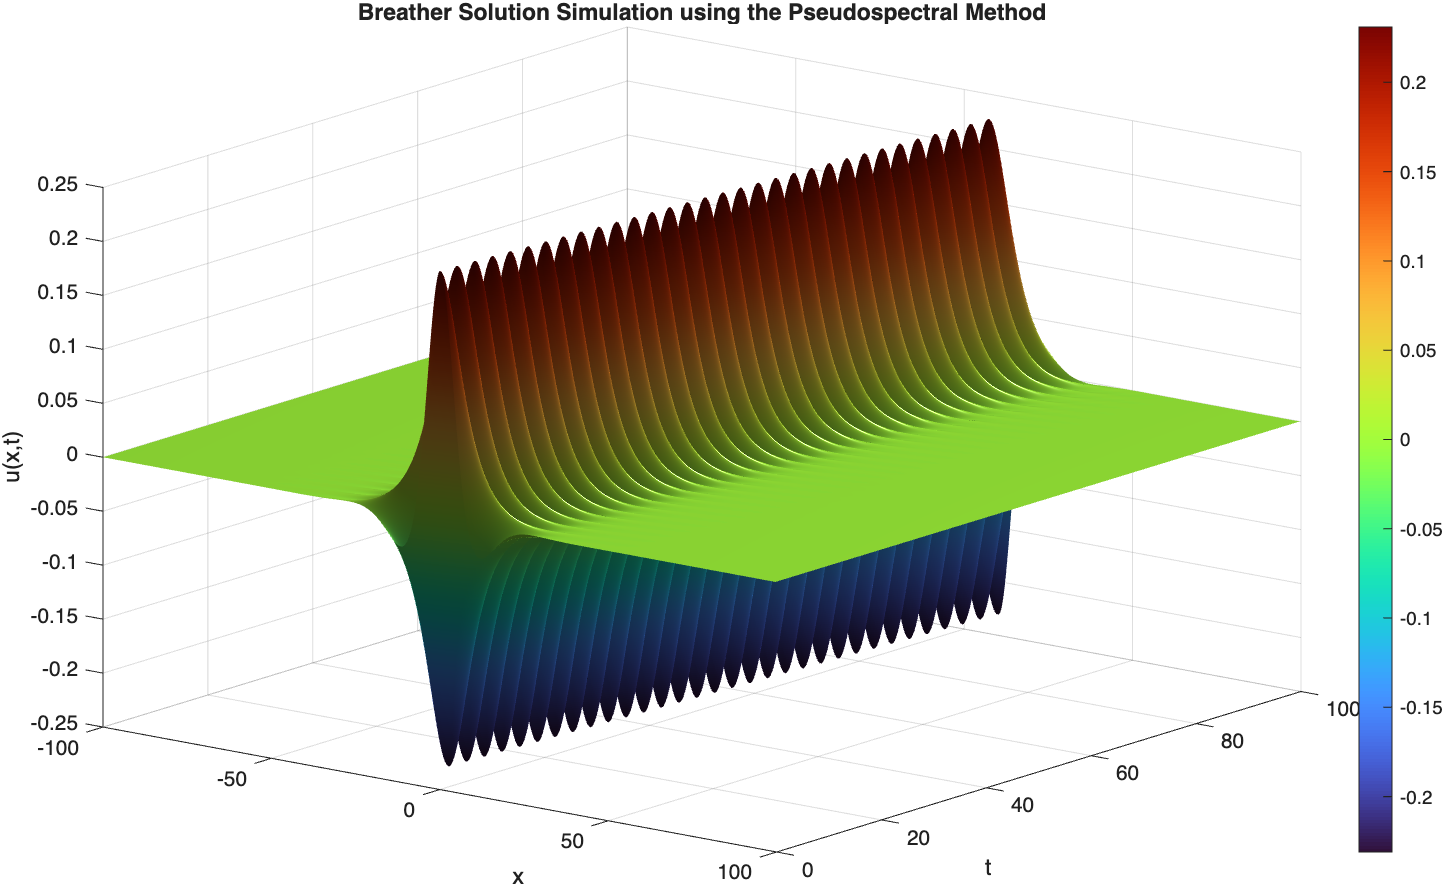
\includegraphics[width=\textwidth]{../plots/pseudospectral1.png}
        \caption{Side view.}
        \label{fig:single_breather_side}
    \end{subfigure}
    \hfill
    \begin{subfigure}[b]{0.48\textwidth}
        \centering
        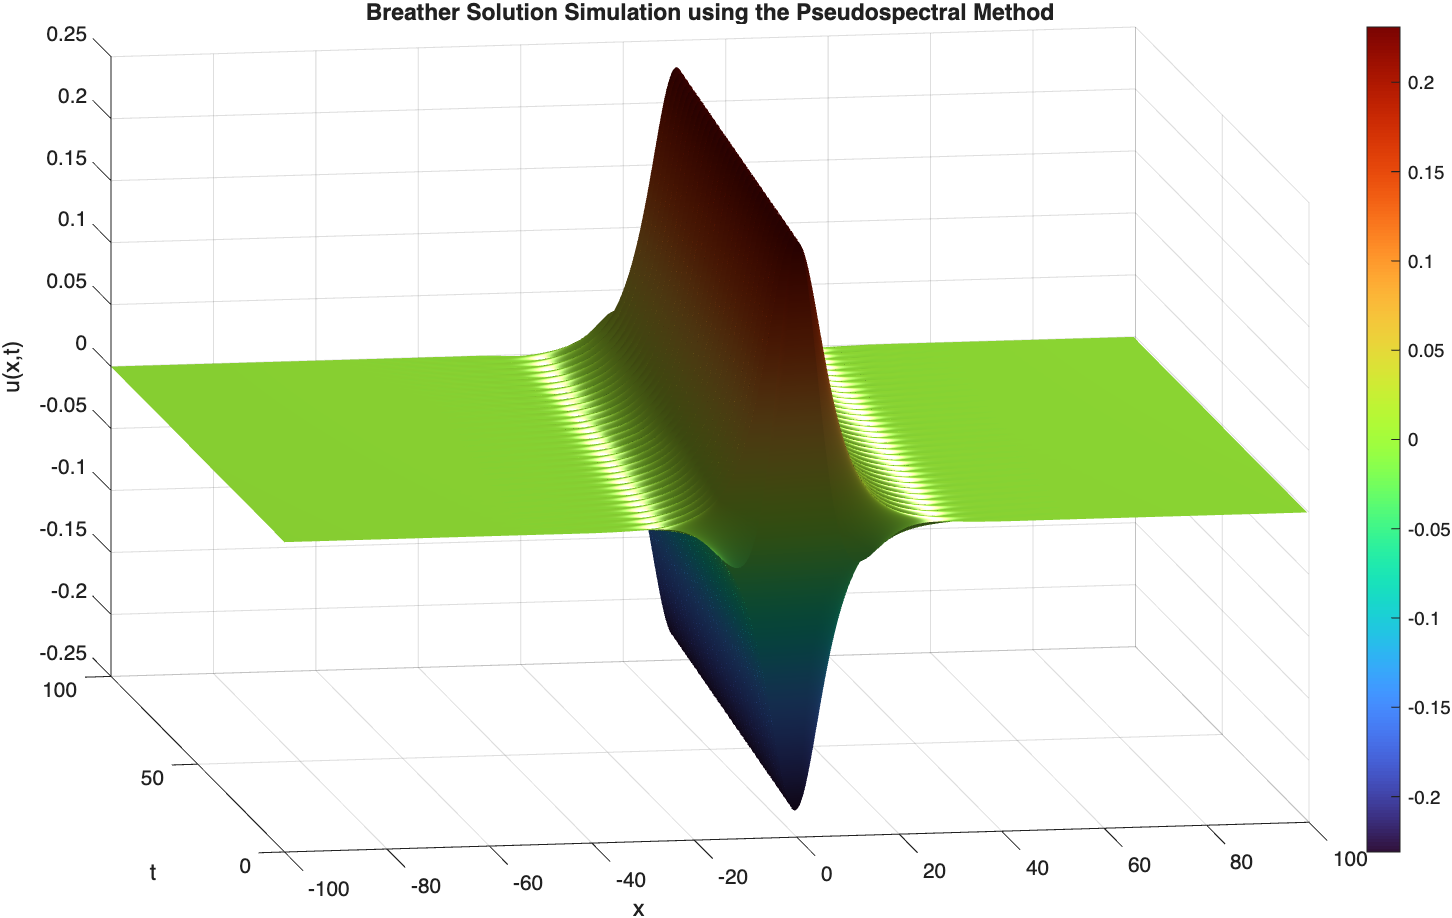
\includegraphics[width=\textwidth]{../plots/pseudospectral2.png}
        \caption{Front view.}
        \label{fig:single_breather_topdown}
    \end{subfigure}

    \caption{Simulation of a single breather solution of the nonlinear Klein-Gordon equation using the pseudospectral method.}
    \label{fig:single_breather}
\end{figure}

We note that we also simulate the solution using an animation, although we do not provide the animation here for obvious reasons. From the animation, we observe that the solution remains highly localised, oscillating between a positive peak and a negative trough centered around $x=0$. In particular, the breather solution repeatedly ``bounces" between these extrema while remaining in the interval of $x \in [-20,20]$, centered about $x=0$. Outside of this region, the solution rapidly decays toward zero and remains approximately flat for the remainder of our chosen domain .\\

Moreover, we observe that the solution does not appear to lose energy throughout the runtime of the simulation, since both the peak amplitudes and trough amplitudes maintain approximately constant magnitudes over time. 

\section*{Head-On Collision of Two Breathers}

Subsequently, we consider how two breather solutions interact with one another. In particular, we study the collisions of two breathers separated by a sufficiently large distance. We are given that the initial condition for the two breathers is given by the following sum:
\[
u(x,0) = A_1\cos(k_1(x-d))\sech\left(\frac{x-d}{b_1}\right)
+ A_2\cos(k_2(x+d))\sech\left(\frac{x+d}{b_2}\right),
\]
moreover, we have the initial velocity given by:
\begin{align*}
u_t(x,0) = {} &
A_1(\omega + k_1v_1)\sin(k_1(x-d))
\sech\left(\frac{x-d}{b_1}\right) \\
&+
A_1\frac{v_1}{b_1}\cos(k_1(x-d))
\sech\left(\frac{x-d}{b_1}\right)
\tanh\left(\frac{x-d}{b_1}\right) \\
&+
A_2(\omega + k_2v_2)\sin(k_2(x+d))
\sech\left(\frac{x+d}{b_2}\right) \\
&+
A_2\frac{v_2}{b_2}\cos(k_2(x+d))
\sech\left(\frac{x+d}{b_2}\right)
\tanh\left(\frac{x+d}{b_2}\right).
\end{align*}

Here, \(A_1\), \(b_1\), and \(k_1\) are of the same form as the parameters \(A\), \(b\), and \(k\), except using the velocity \(v_1\), whilst \(A_2\), \(b_2\), and \(k_2\) are computed using the velocity \(v_2\). Moreover, all the other parameters such as $L=100$, $N=512$ and $\omega=1.98$, remain the same as previously. In our simulations, we choose:
\[
v_1 = 0.1, \qquad v_2 = -0.1,
\]
so that the two breathers initially move towards one another. Moreover, we note that \(d\) represents half of the separation distance between the two breather solutions.\\

In terms of solving for the solution \(u(x,t)\), we follow the same pseudospectral procedure as described previously, except now using the modified initial conditions prescribed above.\\

\subsection*{Case 1: Zero Initial Separation, \(d=0\)}

We start with evaluating $d=0$: 

\begin{figure}[H]
    \centering

    \begin{subfigure}[b]{0.48\textwidth}
        \centering
        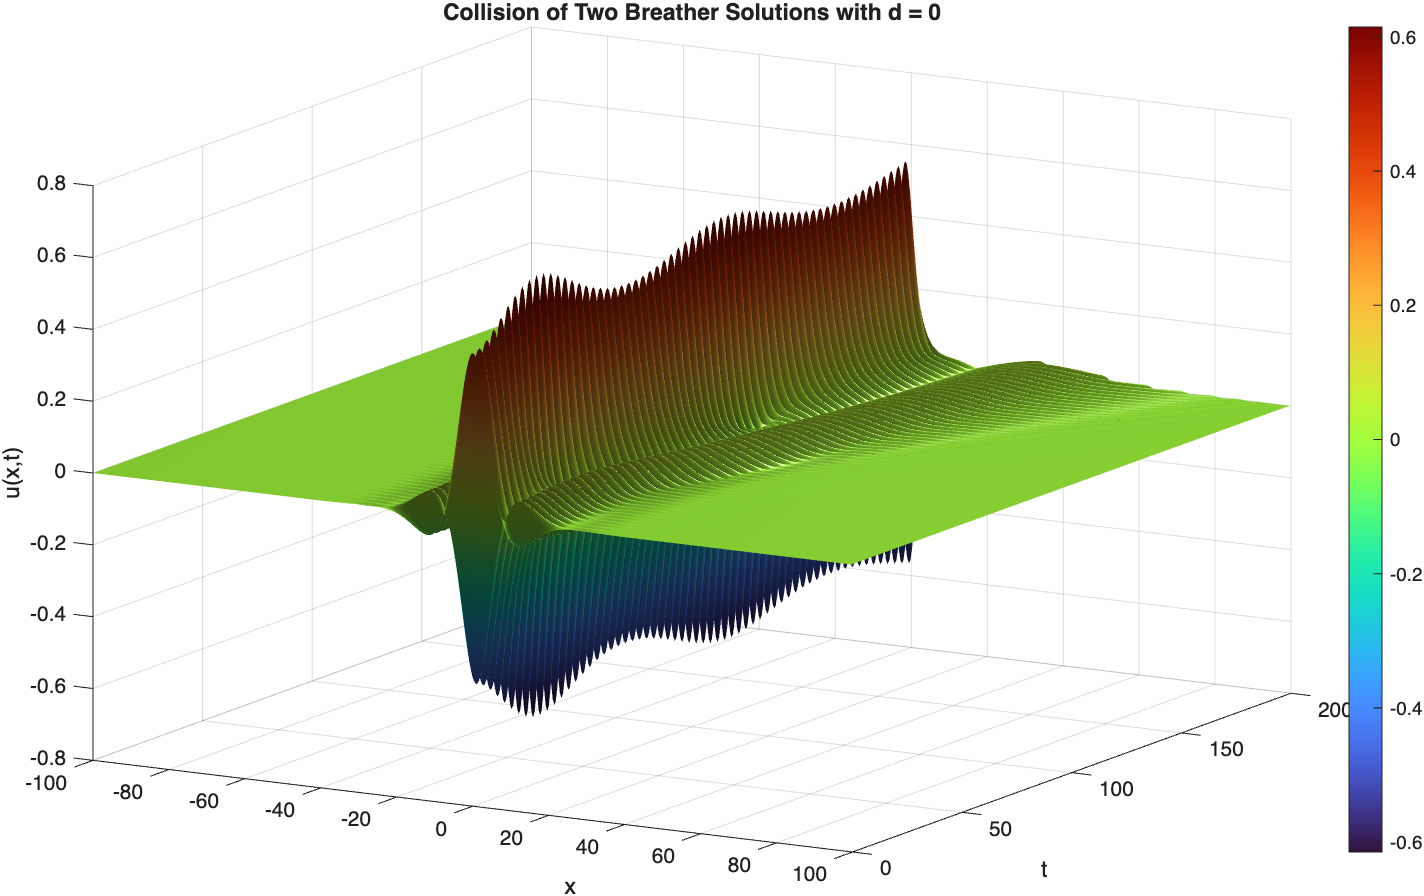
\includegraphics[width=\textwidth]{../plots/breather0.png}
        \caption{Side view of the breather collision for \(d=0\).}
        \label{fig:breather0_side}
    \end{subfigure}
    \hfill
    \begin{subfigure}[b]{0.48\textwidth}
        \centering
        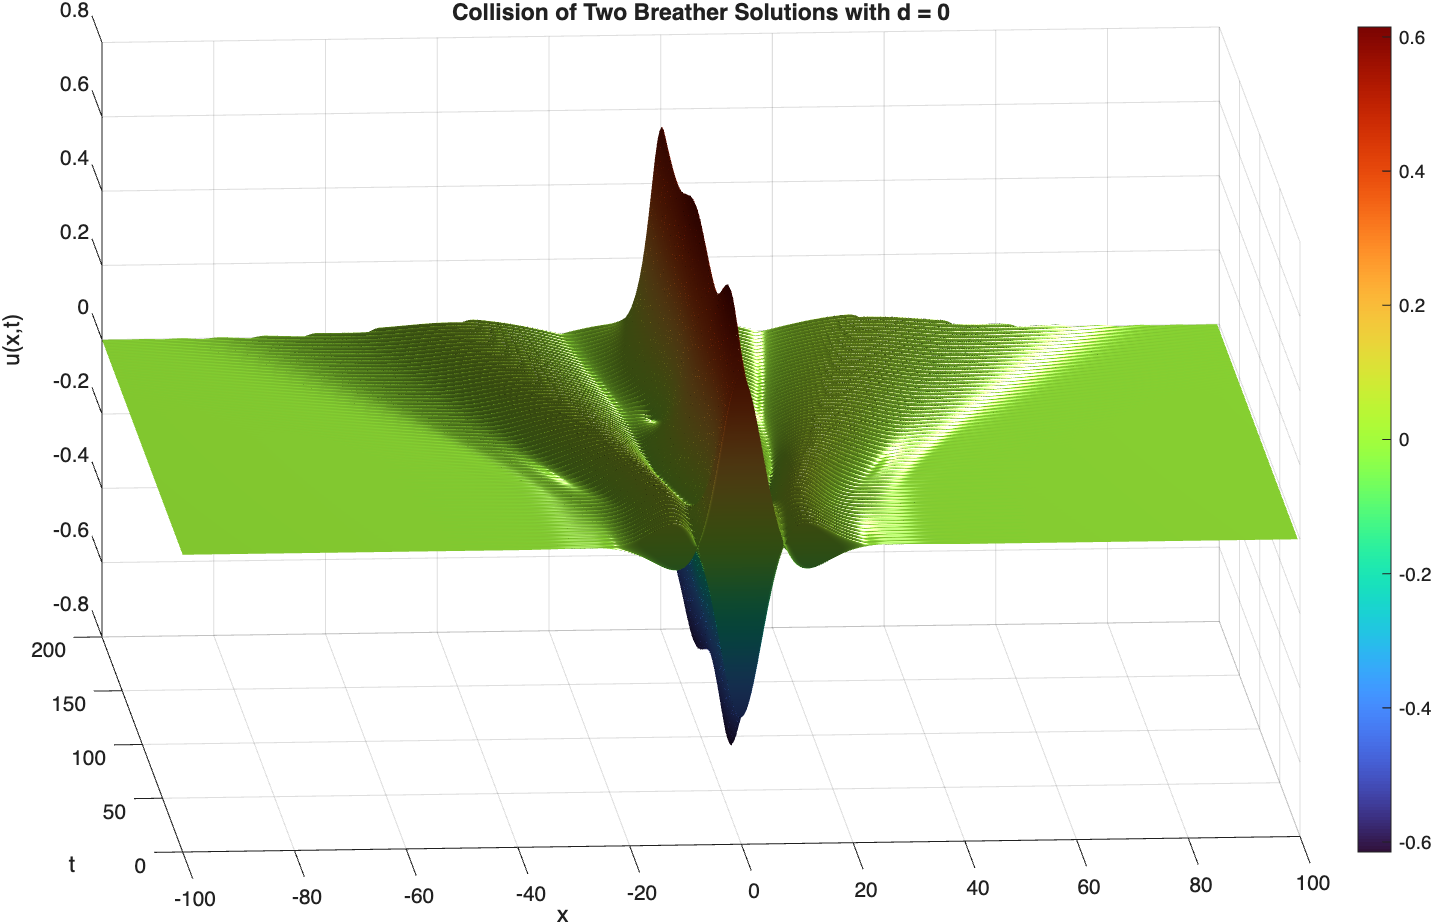
\includegraphics[width=\textwidth]{../plots/breather0topdown.png}
        \caption{Front view of the breather collision for \(d=0\).}
        \label{fig:breather0_front}
    \end{subfigure}

    \caption{Collision of two breather solutions for zero initial separation distance, \(d=0\).}
    
    \label{fig:breather_collision_d0}
\end{figure}

From the simulation for \(d=0\), we observe that the two breather solutions begin completely superimposed at the centre of our domain $[-L,L]$, at $x=0$. As time evolves, we see that the solution remains quite localised around the centre, whilst oscillating periodically between positive and negative amplitudes.\\ 

Moreover, we observe that the collision produces a significantly larger amplitude near the centre of the domain compared to the single breather solution, as we saw previously, which indicates a strong nonlinear effect between the collision of the two breathers. We note that as time progresses, the dynamics appear to remain localised in space, since we have very small amount of dispersement symmetrically about the centre of the domain, which then decays rapidly toward zero.\\

We note that when extending the simulation time beyond \(t=500\), for which we additionally ran an animation of the solution, there appeared to be some Gibbs-like phenomenon occurring near the endpoints of the spatial interval. In particular, oscillatory behaviour began to emerge near the boundaries of the domain, which we assume is due to the periodic boundary conditions. Moreover, after a sufficiently long time, we observed that the breather solution began propagating symmetrically back toward the centre of the domain, namely \(x=0\), and the cycle repeats itself due to the periodic nature of the boundary conditions.\\

\subsection*{Case 2: Half-Separation Distance \(d=20\)}

Next we evaluate the interaction with half-separation of $d=20$:

\begin{figure}[H]
    \centering

    \begin{subfigure}[b]{0.48\textwidth}
        \centering
        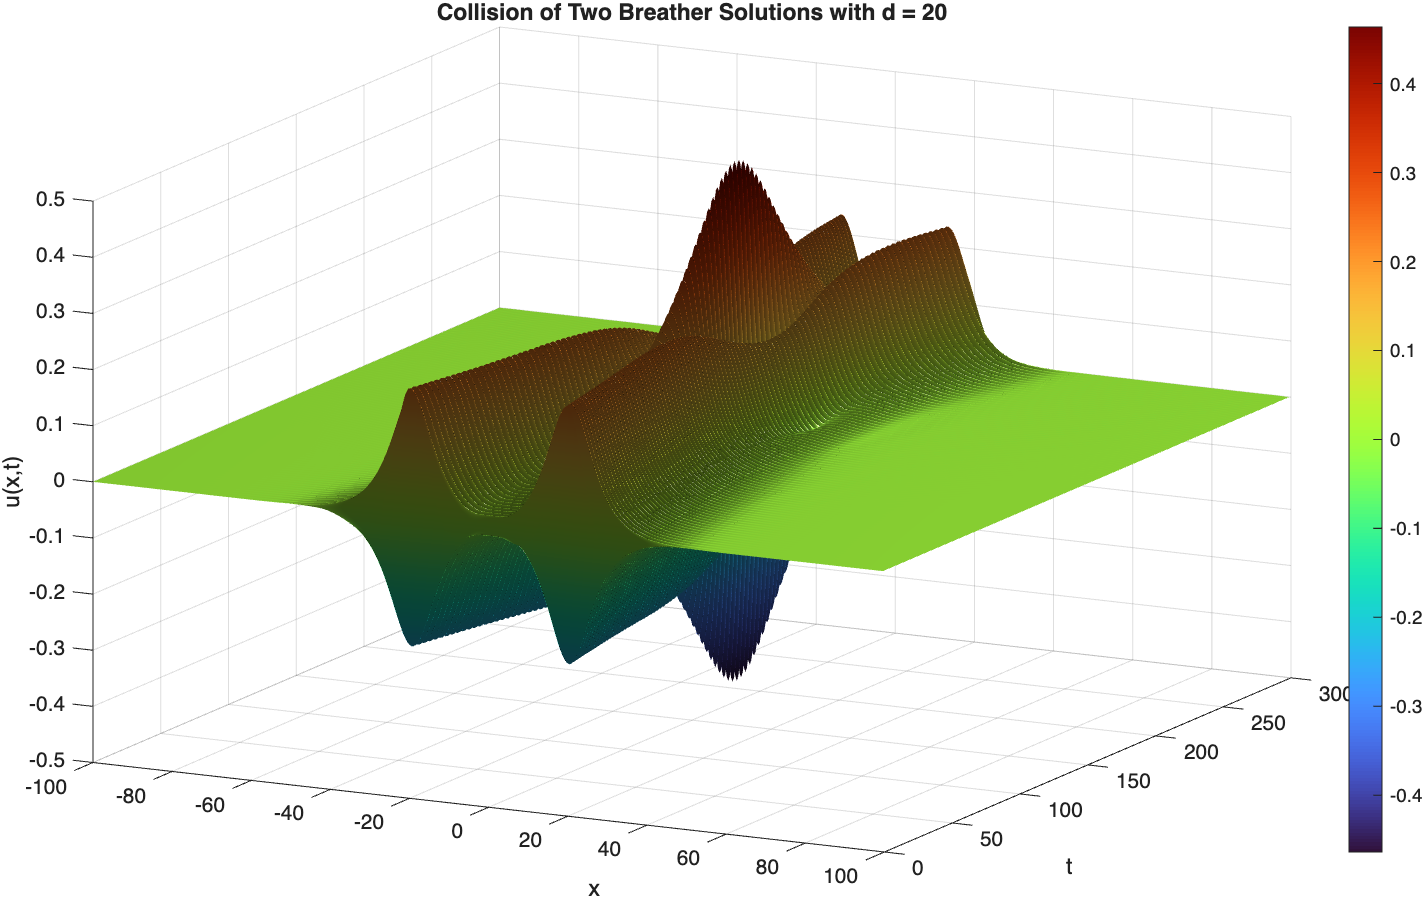
\includegraphics[width=\textwidth]{../plots/breather20.png}
        \caption{Side view of the breather collision for \(d=20\).}
        \label{fig:breather20_side}
    \end{subfigure}
    \hfill
    \begin{subfigure}[b]{0.48\textwidth}
        \centering
        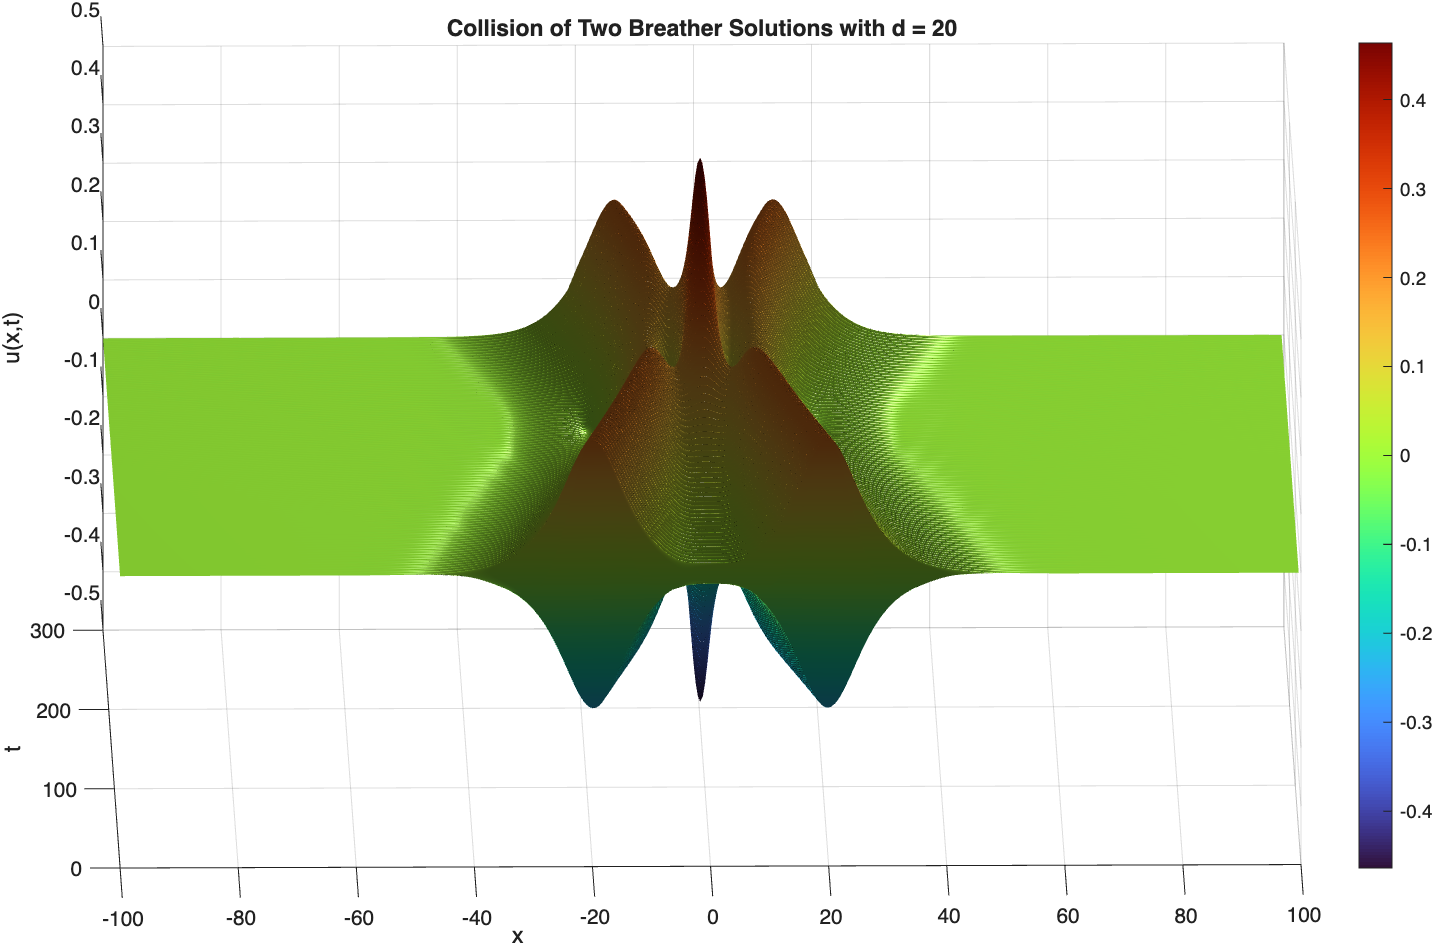
\includegraphics[width=\textwidth]{../plots/breather20_topdown.png}
        \caption{Front view of the breather collision for \(d=20\).}
        \label{fig:breather20_front}
    \end{subfigure}

    \caption{Collision of two breather solutions with half-separation distance \(d=20\).}
    
    \label{fig:breather_collision_d20}
\end{figure}

We observe that initially the two breather structures, which are separated by a distance of \(40\) spatial units, move towards one another as time progresses. The two localised structures subsequently collide after approximately \(150\) time units. At the point of collision, the two breathers superimpose, producing an amplitude significantly larger in magnitude than that of either individual breather structure.\\

Following the collision for the case \(d=20\), the two breather structures diverge away from one another whilst continuing to oscillate between positive and negative amplitudes. We observe that this post-collision motion is approximately symmetric about the centre of the spatial domain, \(x=0\). That is, the two breathers move away from the centre in opposite directions, remaining approximately equidistant from \(x=0\) as they propagate.\\

The two structures continue to diverge until they reach the endpoints of the spatial interval \([-L,L]\), where there appears to be, once again, some Gibbs-like phenomenon. Due to the periodic boundary conditions, they then begin to move back towards one another, again propagating towards the centre of the domain. Once the two breathers return to approximately the same separation distance of \(40\) spatial units, corresponding to a half-separation distance of \(d=20\), they begin moving towards one another again and the collision cycle repeats. This recurring behaviour was confirmed through an animation of the solution run beyond \(t=800\).\\

\subsection*{Case 3: Half-Separation Distance \(d=35\)}

For the interaction with half-separation distance of $d=35$ we obtain the following:\\

\begin{figure}[H]
    \centering

    \begin{subfigure}[b]{0.48\textwidth}
        \centering
        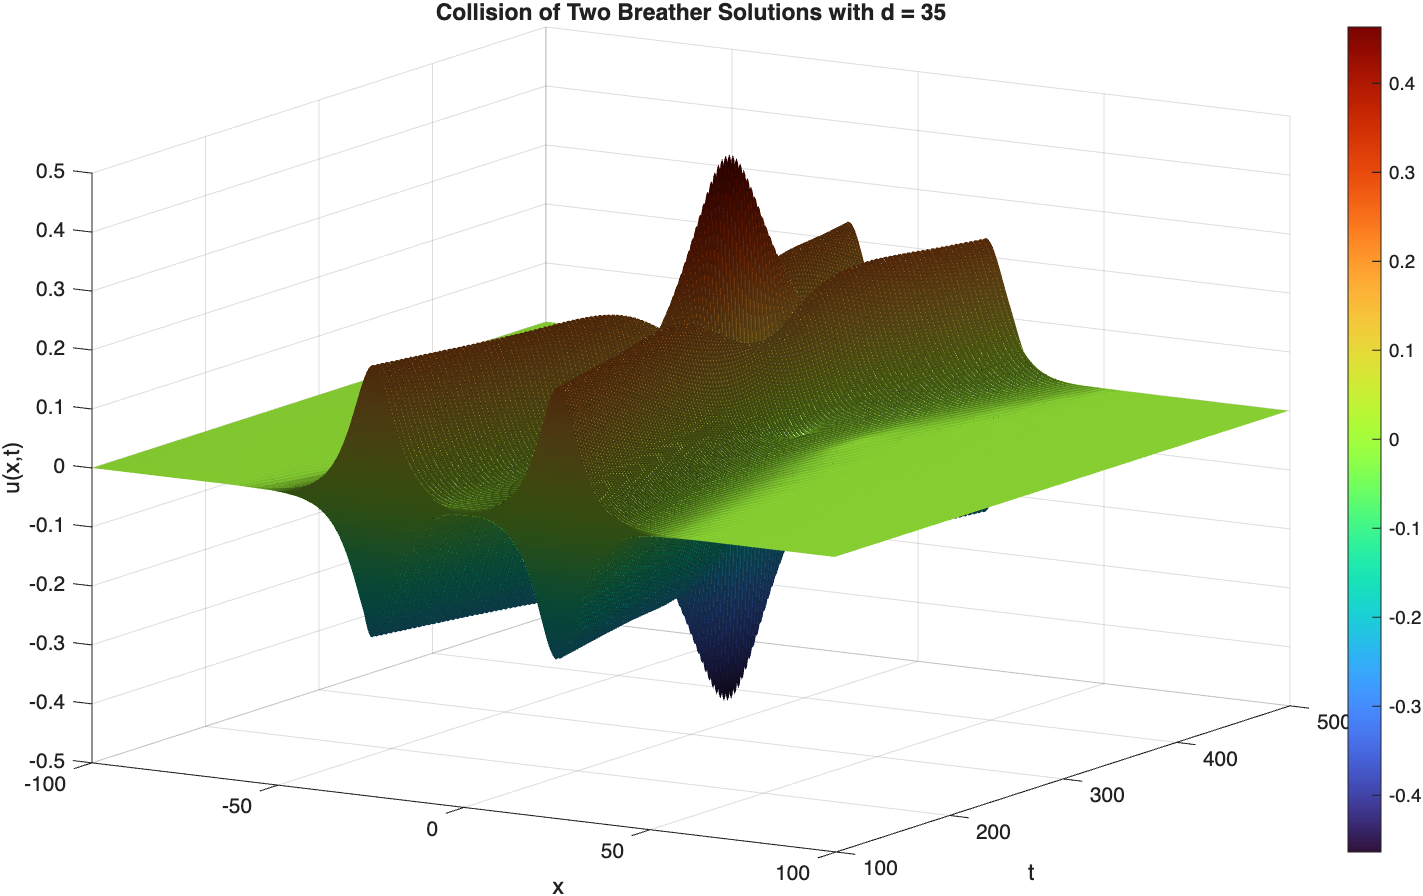
\includegraphics[width=\textwidth]{../plots/breather35.png}
        \caption{Side view of the breather collision for \(d=35\).}
        \label{fig:breather35_side}
    \end{subfigure}
    \hfill
    \begin{subfigure}[b]{0.48\textwidth}
        \centering
        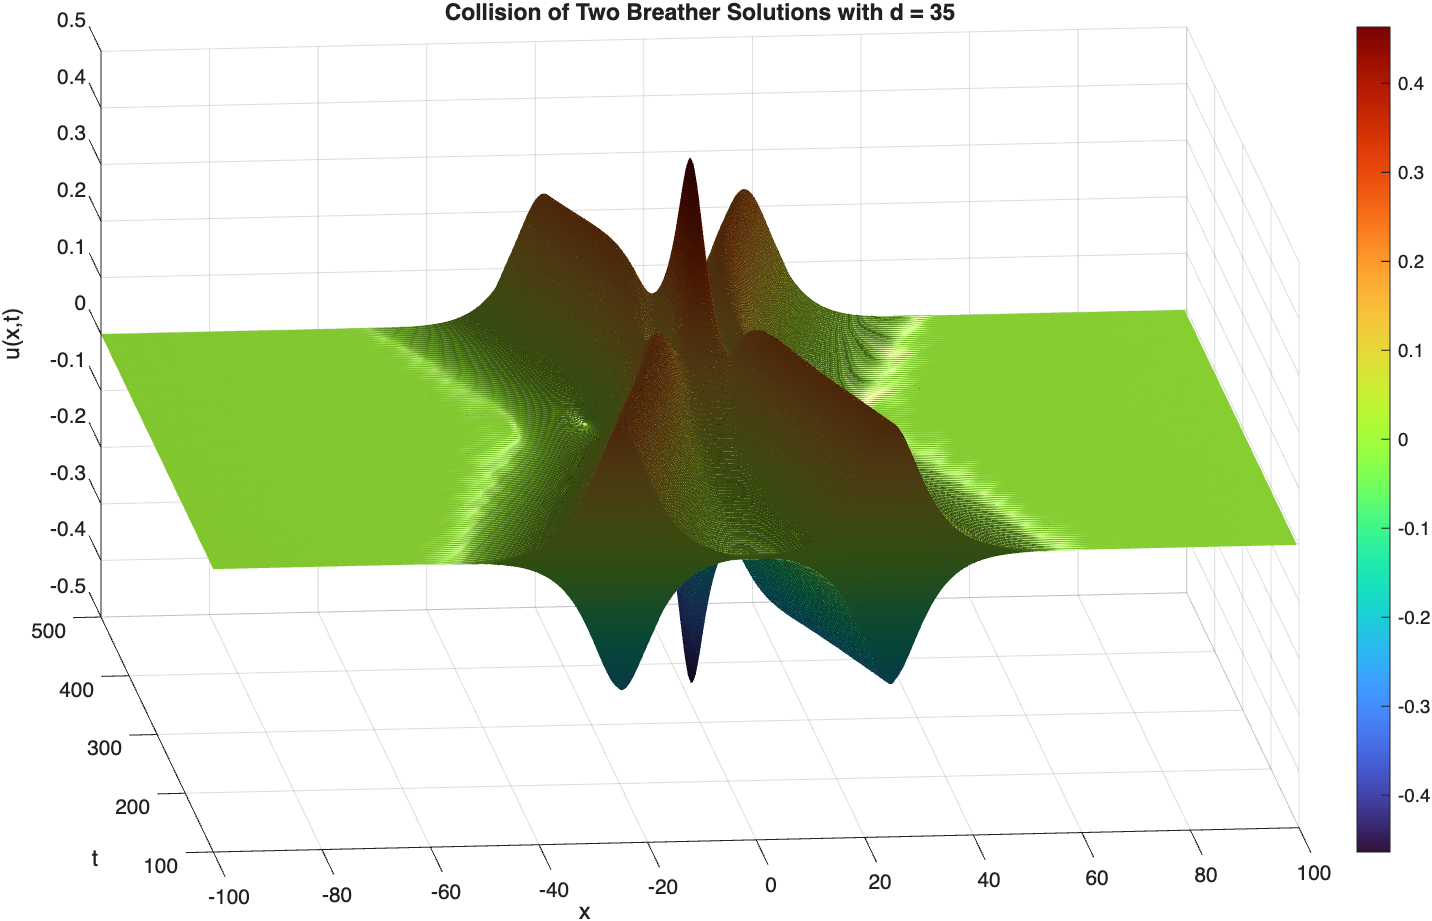
\includegraphics[width=\textwidth]{../plots/breather35_topdown.png}
        \caption{Front view of the breather collision for \(d=35\).}
        \label{fig:breather35_front}
    \end{subfigure}

    \caption{Collision of two breather solutions with half-separation distance \(d=35\). }
    
    \label{fig:breather_collision_d35}
\end{figure}

When setting the half-separation distance to be \(d=35\), we note that the breather structures show similar behaviour to the case where \(d=20\). However, since the two breathers are initialised further apart from one another, they take a longer time to collide. In this case, the collision occurs at approximately \(t=300\).\\

Moreover, we observe that the amplitude magnitudes of the individual breather structures are approximately the same as in the previous case. When the two breathers collide, they once again superimpose to produce an amplitude that is larger in magnitude than either of the individual breather structures.\\

After the collision occurs, the two breathers diverge away from one another, oscillating back and forth as they propagate. This post-collision motion is approximately symmetric about the centre of the spatial domain, \(x=0\). The two structures continue moving apart until they approach the endpoints of the interval \([-L,L]\), where we observe some Gibbs-like oscillatory behaviour near the boundaries. Due to the periodic boundary conditions, the breathers then begin moving back towards one another.\\

Once the two breathers return to approximately their initial half-separation distance of \(d=35\), the collision cycle repeats itself. This recurring behaviour was confirmed through several  animations run beyond \(t=1000\).\\

\subsection*{Case 4: Half-Separation Distance \(d=50=L/2\)}

Finally for $d=50$, which is $d=L/2$ in this case since $L=100$, we have that:\\

\begin{figure}[H]
    \centering

    \begin{subfigure}[b]{0.48\textwidth}
        \centering
        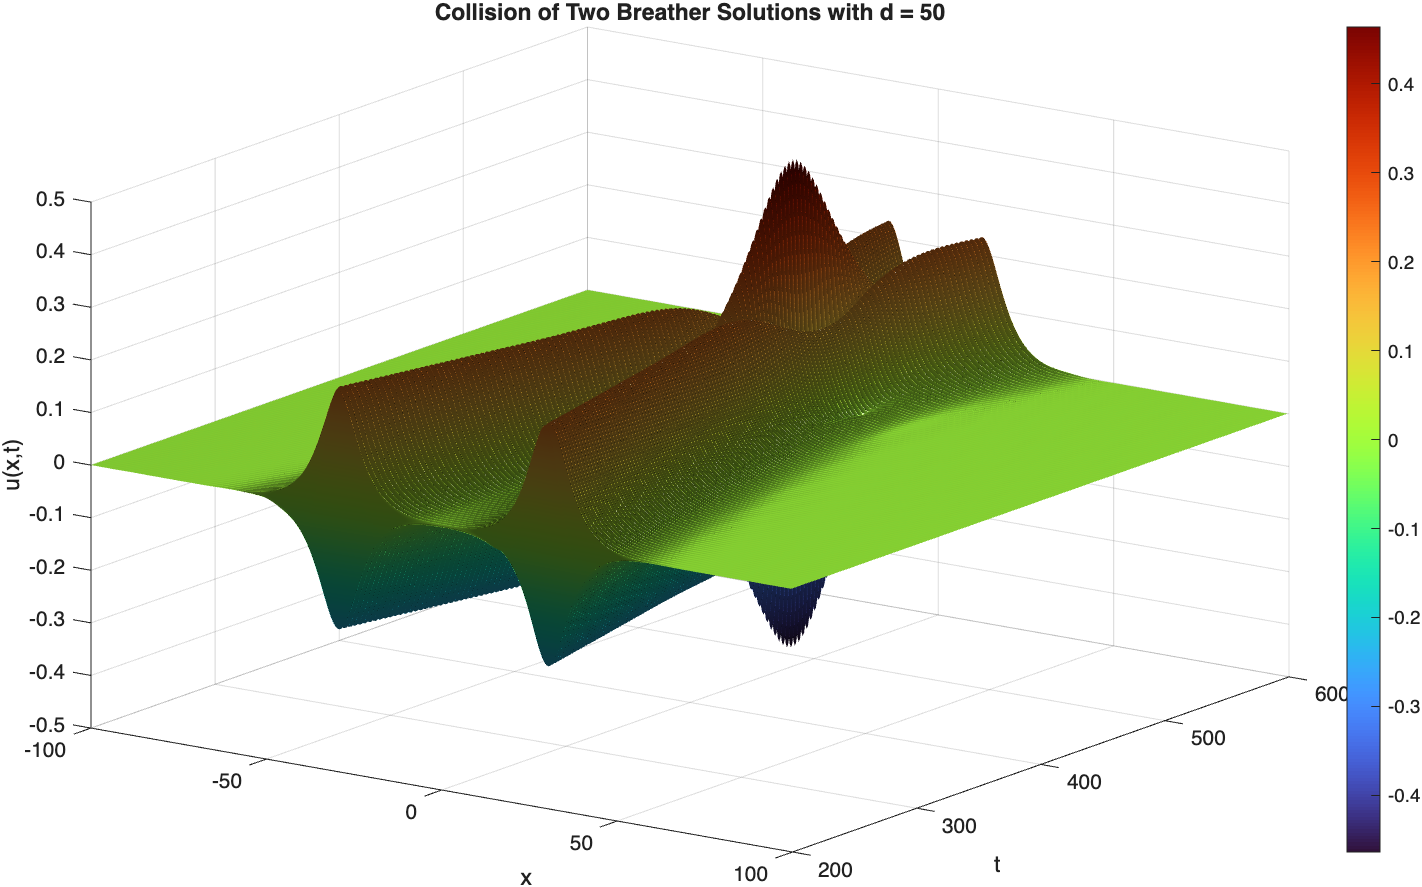
\includegraphics[width=\textwidth]{../plots/breather50.png}
        \caption{Side view of the breather collision for \(d=50\).}
        \label{fig:breather50_side}
    \end{subfigure}
    \hfill
    \begin{subfigure}[b]{0.48\textwidth}
        \centering
        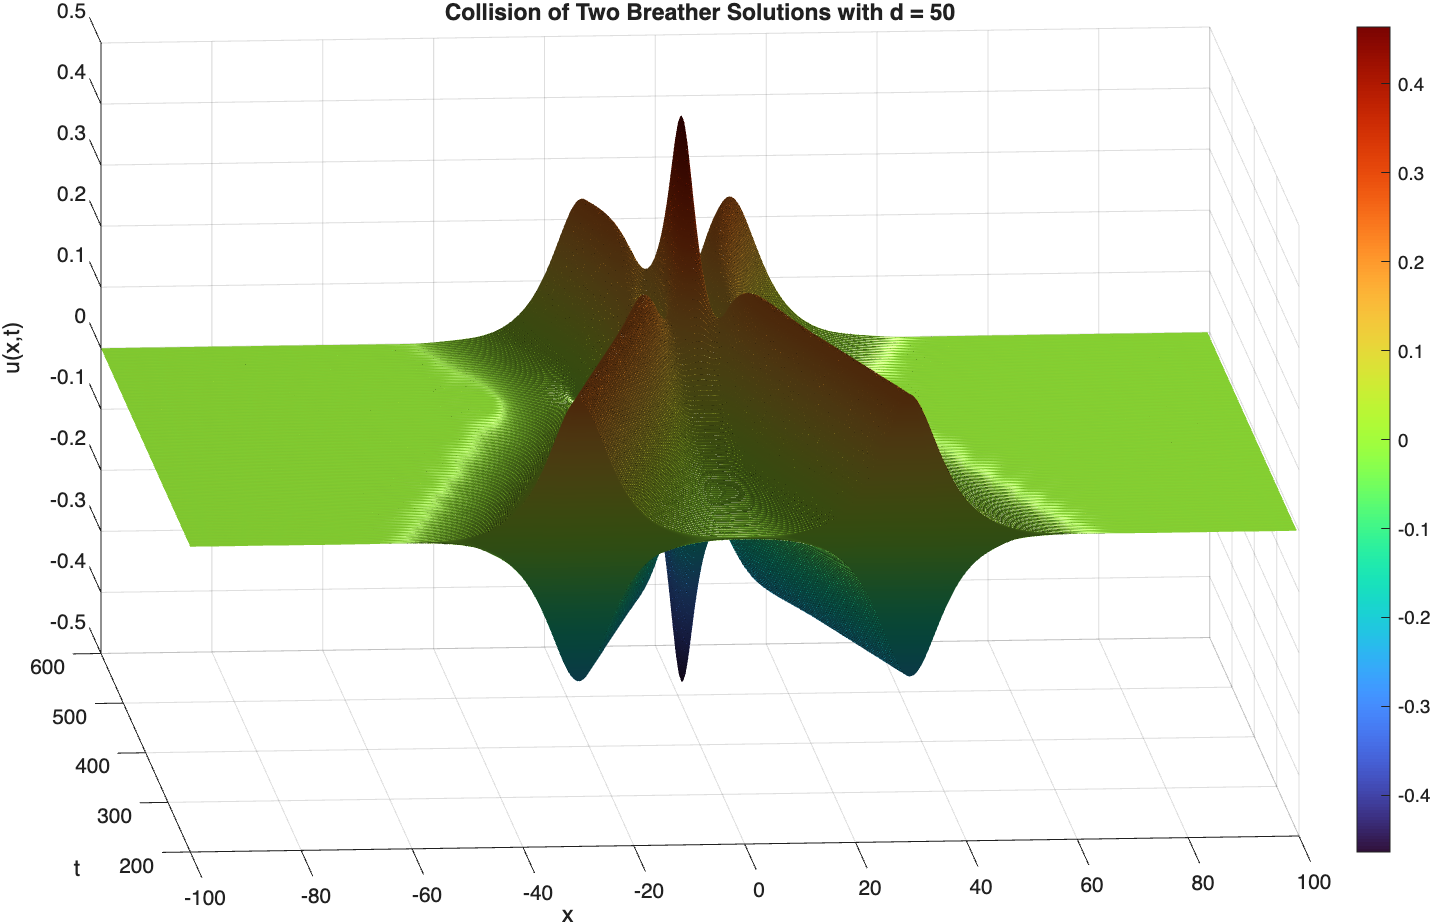
\includegraphics[width=\textwidth]{../plots/breather50_topdown.png}
        \caption{Front view of the breather collision for \(d=50\).}
        \label{fig:breather50_front}
    \end{subfigure}

    \caption{Collision of two breather solutions with half-separation distance \(d=50\).}
    
    \label{fig:breather_collision_d50}
\end{figure}

We note that once again the breather structure is very similar to the cases \(d=20\) and \(d=35\), except now the initial half-separation distance is \(d=50\). Since the breathers are initially placed quite far apart, the collision occurs much later, at approximately \(t=500\). For computational efficiency, we truncate the plot so that it begins at \(t=200\), which is still well before the collision takes place.\\

We observe that the breather solutions once again oscillate towards one another and then collide. At the point of collision, they superimpose, producing an oscillating amplitude that is much greater than the oscillating amplitude of each individual breather component. Post-collision, the breather components diverge symmetrically away from one another, moving towards the endpoints of the spatial interval.\\

Moreover, near the endpoints, we observe some Gibbs-like phenomenon, which appears as oscillatory behaviour close to the boundaries of the interval. Once the breathers reach the endpoints, they begin moving towards one another again, eventually returning to approximately their initial half-separation distance with their original amplitudes. Thus, the cycle continues. This recurring behaviour was confirmed through several animations of the solution run beyond \(t=1500\). \\

\subsection*{Quantitative Comparison of Collision Amplitudes}

Now, in order to quantify the interaction of the breathers, we record the largest magnitude reached by the amplitude of the solution at the time just after the collision. We then plot this collision amplitude against the corresponding value of the half-separation distance \(d\):

\begin{figure}[H]
    \centering
    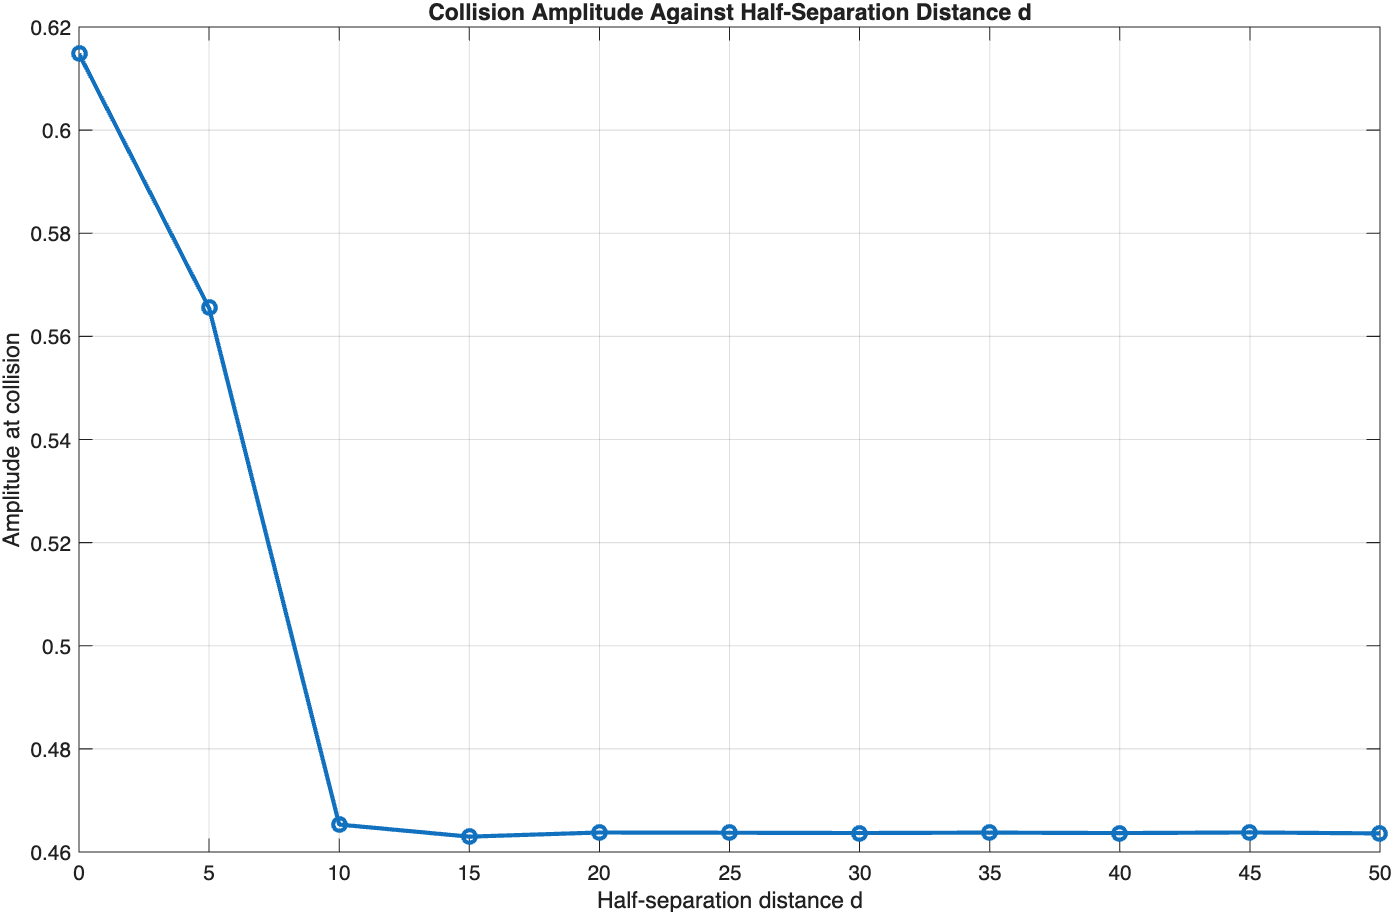
\includegraphics[width=0.85\textwidth]{../plots/collisionamplitudeplot.png}
    \caption{Maximum amplitude reached by the solution at the time just after collision, plotted against the half-separation distance \(d\).}
    \label{fig:collision_amplitude_vs_d}
\end{figure}

From the quantitative data, we observe that when the two breathers collide with no initial separation distance, \(d=0\), the collision produces the largest amplitude. In this case, the maximum amplitude at collision is approximately \(0.618\), indicating that the strongest interaction occurs when the two breather structures are initially superimposed.\\

As the half-separation distance \(d\) is increased, the maximum collision amplitude decreases. This decrease is most significant between \(d=0\) and \(d=10\). After approximately \(d=10\), the maximum amplitude at collision appears to stabilise at around \(0.465\). Thus, beyond this point, increasing the initial half-separation distance does not appear to significantly affect the maximum amplitude produced at the collision.\\

\section*{Conclusion}

In this project, we implemented a pseudospectral method to simulate breather solutions of the nonlinear Klein-Gordon equation. The spatial derivative was computed in Fourier space using the Fast Fourier Transform, while the time evolution was performed using a centered finite difference scheme. Since the centered difference method requires two initial time levels, we used a Taylor expansion about \(t=0\) to construct the first time step from the prescribed initial displacement and initial velocity.\\

The single breather simulation confirmed the expected qualitative behaviour of a breather solution. Namely, the solution remained strongly localised around the centre of the domain and oscillated between positive and negative amplitudes without appearing to lose amplitude over the runtime of the simulation.\\

We then studied the interaction of two breathers undergoing head-on collisions for different values of the half-separation distance \(d\). For \(d=0\), the two breathers were initially superimposed, resulting in the largest observed amplitude. For \(d=20\), \(d=35\), and \(d=50\), the breathers began separated from one another, propagated towards the centre of the domain, collided, and then moved away from one another approximately symmetrically. In each of these cases, the collision produced a larger amplitude than that of either individual breather component, thus demonstrating the nonlinear nature of the interaction.\\

The quantitative amplitude plot showed that the maximum collision amplitude decreases as the initial half-separation distance \(d\) increases. This decrease is strongest between \(d=0\) and approximately \(d=10\). Beyond this point, the amplitude stabilises at approximately \(0.465\), suggesting that once the breathers are sufficiently separated initially, increasing \(d\) has little effect on the maximum amplitude produced at collision.\\

Overall, the simulations show that the pseudospectral method provides an effective way to study localised nonlinear wave interactions. The results suggest that the initial separation distance plays an important role when the breathers are close together, but has a much weaker effect once the breathers are sufficiently far apart. Finally, the periodic boundary conditions also play an important role in the long-time behaviour, since we note that they cause the breathers to re-enter the domain and collide again after reaching the boundaries.

\appendix
\section{MATLAB Code for the Pseudospectral Method}

\begin{lstlisting}[language=Matlab, caption={Implementation of the pseudospectral method for the nonlinear Klein-Gordon equation}, label={lst:pseudospectral}]
clc
clear
close all

% Here we implement the pseudospectral method for the nonlinear
% Klein-Gordon Equation: u_tt -4u_xx + f(u) = 0, where f(u) = 4u -2u^3

% params:
omega = 1.98;
v= 0.1;
A = 2/(sqrt(3))*(sqrt(4-(omega)^2/(1-v^2)));
b = 2/sqrt(3)*(sqrt(1-v^2)/A);
k = (v*omega)/(1-v^2);

% now we set up our spatial grid: 
L = 100;
N = 512; % we recall that using a power of 2 for fft is most efficient. 
h = (2*L)/N; % since we are working on a spatial grid of [-L,L]
               % thus total length is 2L
x = (-N/2: N/2-1)*h;

% we find our Fourier wave numbers, and recall that we are working on an
% interval of [-L,L], thus we have 2pi.n/2L = (pi/L).n
q = (pi/L)*[0:N/2-1 -N/2:-1];

% we then setup our temporal grid: 
tau = 0.01;
T = 100;
Num_time_steps = round(T/tau);

% we introduce our initial conditions as follows: 
u_0 = A*cos(k*x).*sech(x/b);

u_t0 = A*(omega+(k*v))*sin(k*x).*sech(x/b)...
    + A*v/b*cos(k*x).*sech(x/b).*tanh(x/b);

% we then compute our spatial values in Fourier space, using u_0: 
u_hat = fft(u_0);
u_xx0 = real(ifft(-(q.^2).*u_hat));

% next we compute u_tt(0) by subbing into our original equation: 
u_tt0 = u_xx0 - 4*u_0 + 2*u_0.^3;

% then we find the Taylor expansion of u(x,tau), which shall give us the
% next value of u in time, which we need for the central difference
% approximation, since the scheme is a 3 level time scheme: 
u_old = u_0;
u = u_0 + tau*u_t0 + (tau^2/2)*u_tt0;

% we instantiate a matrix U, which shall store the vectors of u for every
% point in time, and T_vals stores the corresponding time value for the
% time index of u: 
U = [];
T_vals = [];

for n = 1:Num_time_steps
   
    u_hat = fft(u);
    u_xx = real(ifft(-(q.^2).*u_hat));
    
    % we use the centre difference to update in time: 
    u_new = 2*u - u_old + tau^2*(u_xx - 4*u + 2*u.^3);
    
    u_old = u;
    u = u_new;
    
    % we store the values within arrays in order to plot: 
    U = [U; u];
    T_vals = [T_vals; n*tau];
    
end
 
% finally we plot the solution: 
[X, TT] = meshgrid(x, T_vals);

figure;
surf(X, TT, U, 'EdgeColor', 'none',...
	'FaceColor', 'interp');
xlabel('x');
ylabel('t');
zlabel('u(x,t)');
title('Breather Solution Simulation using the Pseudospectral Method');
view(45,35);
colormap(turbo);
colorbar;
shading interp;
camlight;
lighting gouraud;

% here is our code for the animation of the breather solution: 
%figure;

%for j = 1:length(T_vals)

    %plot(x, U(j,:), 'LineWidth', 2);
    %xlabel('x');
    %ylabel('u(x,t)');
    %title(['animation of Breather Solution:', num2str(T_vals(j), '%.2f')]);

    %ylim([min(U(:)) max(U(:))]);
    %xlim([min(x) max(x)]);
    %grid on;

    %drawnow;

%end
\end{lstlisting}

\section{Additional MATLAB Code for Two Breather Interaction}

\begin{lstlisting}[language=Matlab, caption={Initial conditions for the interaction of two breather solutions}, label={lst:two_breather_initial_conditions}]
% extra params for breathers colliding:
omega = 1.98;
v_1 = -0.1;   
v_2 =  0.1;   

A_1 = 2/sqrt(3)*sqrt(4 - omega^2/(1 - v_1^2));
b_1 = 2/sqrt(3)*sqrt(1 - v_1^2)/A_1;
k_1 = v_1*omega/(1 - v_1^2);

A_2 = 2/sqrt(3)*sqrt(4 - omega^2/(1 - v_2^2));
b_2 = 2/sqrt(3)*sqrt(1 - v_2^2)/A_2;
k_2 = v_2*omega/(1 - v_2^2);

d = 35;

% initial conditions for two solutions interacting: 
u_0 = A_1*cos(k_1*(x-d)).*sech((x-d)/b_1) ...
    + A_2*cos(k_2*(x+d)).*sech((x+d)/b_2);

u_t0 = A_1*(omega + k_1*v_1).*sin(k_1*(x-d)).*sech((x-d)/b_1) ...
    + A_1*(v_1/b_1).*cos(k_1*(x-d)).*sech((x-d)/b_1).*tanh((x-d)/b_1) ...
    + A_2*(omega + k_2*v_2).*sin(k_2*(x+d)).*sech((x+d)/b_2) ...
    + A_2*(v_2/b_2).*cos(k_2*(x+d)).*sech((x+d)/b_2).*tanh((x+d)/b_2);
\end{lstlisting}

\section*{References}

\begin{itemize}

\item N.\ V.\ Alexeeva, \textit{MAM3042F: Advanced Numerical Methods Lecture Notes}, 
Department of Mathematics and Applied Mathematics, University of Cape Town, 2026.

\item X.\ Antoine and X.\ Zhao, \textit{Pseudospectral methods with PML for nonlinear Klein-Gordon equations in classical and non-relativistic regimes}, Journal of Computational Physics, vol.\ 448, Article 110728, 2022.

\item \textit{MATLAB Documentation}, The MathWorks, Inc. Available at: \\ \texttt{https://www.mathworks.com/help/} (accessed March 2026).

\end{itemize}
\end{document}